\section{Metodologia.}\label{Metodologia.}

O projeto proposto será composto pelas etapas que seguem (\autoref{fig_fluxo_met}).

\begin{figure}[htb]
	\caption{\label{fig_fluxo_met} Fluxo logístico do envio e retorno de maquinetas, laço fechado}
	\begin{center}
            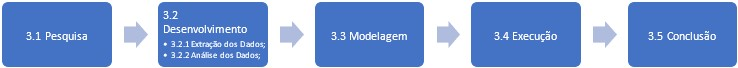
\includegraphics[width=15cm]{images/RF_img/FluxoMetodologia.jpg}
	\end{center}
	\fdadospesquisa
\end{figure}

\subsection[Pesquisa]{Pesquisa}
\label{Pesquisa}
Esta etapa se trata da pesquisa por mais projetos desenvolvidos no assunto abordado, pela revisão bibliográfica de mais artigos e exemplos de sucesso no desenvolvimento e escrita/documentação do que foi estudado.

Esta etapa se trata da pesquisa por mais projetos desenvolvidos no assunto abordado, pela revisão bibliográfica de mais artigos e exemplos de sucesso no desenvolvimento e escrita/documentação do que foi estudado.

\subsection[Desenvolvimento]{Desenvolvimento}
\label{Desenvolvimento}

Para o desenvolvimento do estudo, devido a capacidade computacional, as análises foram reduzidas para o estado de SP como validação do modelo.

\subsubsection[Extração dos Dados]{Extração dos Dados}
\label{Extração dos Dados}

Nesta etapa, foram coletados dados de estados, regiões, regiões imediatas, municípios, latitude, longitude e população por município diretamente da \sigla{API}{Interface de Programação de Aplicativos} do \sigla{IBGE}{Instituto Brasileiro de Geografia e Estatística} \cite{ibge:2025:divisoesregionais} (\autoref{tab:dados_municipios}).

\begin{table}[h!]
\centering
\caption{Características das Colunas de Dados dos Municípios Brasileiros}
\label{tab:dados_municipios}
\begin{tabular}{|p{5cm}|p{2cm}|p{2cm}|p{5cm}|} % Ajuste das larguras das colunas
\hline
\textbf{Coluna} & \textbf{Número de Linhas} & \textbf{Tipo} & \textbf{Descrição} \\
\hline
uf & 645 & object & Sigla do estado \\
\hline % Linha adicionada
regiao & 645 & object & Região do Brasil \\
\hline % Linha adicionada
codigo\_ibge & 645 & object & Código único do município \\
\hline % Linha adicionada
nome\_cidade & 645 & object & Nome da cidade \\
\hline % Linha adicionada
latitude\_cidade & 645 & float64 & Latitude da cidade \\
\hline % Linha adicionada
longitude\_cidade & 645 & float64 & Longitude da cidade \\
\hline % Linha adicionada
Nome do Município & 645 & object & Nome da cidade \\
\hline % Linha adicionada
Nome da Região Imediata & 645 & object & Nome da região geográfica imediata \\
\hline % Linha adicionada
Nome do Município da Região Imediata & 645 & object & Nome do principal município da região geográfica imediata \\
\hline % Linha adicionada
Pop\_2022 & 645 & float64 & População estimada para 2022 \\
\hline
\end{tabular}
\end{table}

\subsubsection[Geração de Dados e Definições de Parâmetros]{Geração de Dados e Definições de Parâmetros}
\label{Geração de Dados}\par

Foram gerados os dados de parâmetro, que foram apresentados na seção \ref{Modelagem Matemática}, para que as instâncias sejam testadas. Seguindo a mesma organização da seção apresentada, os dados são separados por clientes, postos avançados, CD e fábrica, com seus respectivos valores por instâncias.

\paragraph[Clientes ZDs]{Clientes ZDs}
\label{Clientes}

Os parâmetros para clientes basicamente são dois: demanda de instalação e demanda de desinstalação \autoref{tab:clientes}. Os dados de demanda estão por latitude e longitude, sendo dados gerados através dos dados de população, que foi extraída conforme na seção \ref{Extração dos Dados}.\par

\begin{table}[h!]
\centering
\caption{clientes}
\label{tab:clientes}
\begin{tabular}{|c|c|c|c|}
\hline
\textbf{Variável} & \textbf{Instância 1} & \textbf{Instância 2} & \textbf{Instância 3} \\
\hline
$dem^{rj}_{j,t}$ & $dem^{rj}_{j,t} \in [0, 1.146M]$ & $dem^{rj}_{j,t} \in [0, 1.172M]$ & $dem^{rj}_{j,t} \in [0, 1.179M]$ \\
\hline
$dem^{aj}_{j,t}$ & $dem^{aj}_{j,t} \in [0, 1.322M]$ & $dem^{aj}_{j,t} \in [0, 1.362M]$ & $dem^{aj}_{j,t} \in [0, 1.367M]$ \\
\hline
\end{tabular}
\end{table}

Inicialmente foi gerado um histograma para classificar os municípios conforme sua população, utilizando a faixa de 50 mil habitantes como critério principal. A visualização dessa classificação pode ser encontrada na Figura \ref{fig_hist_c_sp}.

\begin{figure}[htb]
	\caption{\label{fig_hist_c_sp} Histograma da população do estado de São Paulo}
	\begin{center}
            \includegraphics[width=10cm]{images/RF_img/Pop_c_SP_Hist.png}
	\end{center}
	\fdadospesquisa
\end{figure}

O estado de São Paulo possui uma concentração muito grande e discrepante na capital em relação às outras cidades, tendo sua faixa populacional acima de 12 milhões de habitantes. Com isso, foi necessário um tratamento à parte, sendo criado um novo histograma sem a cidade de São Paulo, utilizando faixa populacional de 25 mil habitantes \autoref{fig_hist_s_sp}.

\begin{figure}[htb]
	\caption{\label{fig_hist_s_sp} Histograma da população do estado de São Paulo sem a capital}
	\begin{center}
            \includegraphics[width=10cm]{images/RF_img/Pop_s_SP_Hist.png}
	\end{center}
	\fdadospesquisa
\end{figure}

A geração da demanda foi realizada através da demanda total de maquinetas, que foi de 20 milhões em um ano; em seguida, a empresa que está sendo analisada possui um \emph{market share} (percentual de participação do mercado) de 30\%, com isso foi aplicado este percentual definindo a demanda anual da empresa em questão. Calcula-se a média mensal e aplica-se uma variação randômica seguindo uma distribuição normal com variação de 10\%.

A demanda considerada foi limitada ao estado de SP devido a restrições computacionais, totalizando cerca de 1,3 milhão de instalações anuais, com média de 110 mil por mês. Em função da LR da cadeia, a demanda de desinstalação é estimada em 80\% da demanda de instalação. A Figura \ref{grafico_demanda_isnt_desinst_01} apresenta as curvas de demanda anual (instalação e desinstalação) para a instância 1.

\begin{figure}[htb]
	\caption{\label{grafico_demanda_isnt_desinst_01} Gráfico de Demanda de Instalação e Desinstalação para o Estado de São Paulo - Instância 1}
	\begin{center}
            \includegraphics[width=10cm]{images/RF_img/Demanda_linha_inst_01.png}
	\end{center}
	\fdadospesquisa
\end{figure}

A Instância 2 simula a sazonalidade de Natal, aplicando um acréscimo de 20\% na demanda de instalação em dezembro. Em função da LR e do volume instalado, a demanda de desinstalação apresenta um aumento correspondente de 20\% em janeiro. O perfil da demanda desta instância está detalhado na Figura \ref{grafico_demanda_isnt_desinst_02}.

\begin{figure}[htb]
	\caption{\label{grafico_demanda_isnt_desinst_02} Gráfico de Demanda de Instalação e Desinstalação para o Estado de São Paulo - Instância 2}
	\begin{center}
            \includegraphics[width=10cm]{images/RF_img/Demanda_linha_inst_02.png}
	\end{center}
	\fdadospesquisa
\end{figure}

Para a instância 3, é aplicado uma sazonalidade para o período de carnaval, ocorrendo um aumento de 20\% na instalação no mês de fevereiro e o mesmo aumento de 20\% na desinstalação de março, em decorrência do aumento ocorrido na instalação no mês anterior (\autoref{grafico_demanda_isnt_desinst_03}).

\begin{figure}[htb]
	\caption{\label{grafico_demanda_isnt_desinst_03} Gráfico de Demanda de Instalação e Desinstalação para o Estado de São Paulo - Instância 3}
	\begin{center}
            \includegraphics[width=10cm]{images/RF_img/Demanda_linha_inst_03.png}
	\end{center}
	\fdadospesquisa
\end{figure}

As demandas foram contabilizadas por cidade, porém para melhorar o processamento computacional, a demanda foi consolidada em ZDs. Para definir essas zonas, foram selecionadas 50\% das cidades com maior demanda e com isso a demanda restante foi redistribuída entre estas cidades proporcionalmente. Com isso houve uma redução em 50\% da base de dados total.

% Desta maneira, a distribuição das ZDs por faixa de demanda é apresentada conforme \autoref{hist_faixa_cidade_01}, percebe-se que 5 ZDs possuem o volume muito alto, enquanto as demais são mais uniformemente distribuídas para a instância 1 e .

% \begin{figure}[htb]
% 	\caption{\label{hist_faixa_cidade_01} Histograma de Cidades por Faixa Demanda }
% 	\begin{center}
%             \includegraphics[width=10cm]{images/RF_img/Faixa_Dem_Cidades_inst_01.png}
% 	\end{center}
% 	\fdadospesquisa
% \end{figure}\par

% \begin{figure}[htb]
% 	\caption{\label{hist_faixa_cidade_02} Histograma de Cidades por Faixa Demanda }
% 	\begin{center}
%             \includegraphics[width=10cm]{images/RF_img/Faixa_Dem_Cidades_inst_02.png}
% 	\end{center}
% 	\fdadospesquisa
% \end{figure}\par

% \begin{figure}[htb]
% 	\caption{\label{hist_faixa_cidade_03} Histograma de Cidades por Faixa Demanda }
% 	\begin{center}
%             \includegraphics[width=10cm]{images/RF_img/Faixa_Dem_Cidades_inst_03.png}
% 	\end{center}
% 	\fdadospesquisa
% \end{figure}\par



\paragraph[Postos Avançados (PAs)]{Postos Avançados (PAs)}
\label{Postos Avançados}

Para os Pontos de Atendimento (PAs), foram identificadas algumas cidades com potencial para implantação, com base nas Regiões Geográficas Imediatas. De acordo com o \citeonline{ibge:2024:compreendendoterritorio}, essas regiões representam áreas cujos habitantes recorrem a centros urbanos próximos para suprir necessidades imediatas, como acesso a emprego, saúde, educação, consumo e serviços públicos. Dentro de cada região imediata, foram selecionadas as duas maiores cidades, obtendo-se um total de 112 cidades conforme apresentado na \autoref{poss_pa_sp}.

\begin{figure}[htb]
	\caption{\label{poss_pa_sp} Mapa com as possíveis cidades para abertura de um PA.}
	\begin{center}
            \includegraphics[width=10cm]{images/RF_img/poss_pa_sp.png}
	\end{center}
	\fdadospesquisa
\end{figure}

Para as instâncias 1,2 e 3, o parâmetro $n^{p}$ (quantidade máxima de aberturas de PAs) foi definido como 70\% do total de cidades elegíveis à instalação de um PA. O parâmetro $e^{p}_{p,t}$ (limite máximo de máquinas em estoque) foi determinado individualmente para cada possível PA, com base na faixa de demanda da respectiva região imediata, sendo fixado em 125\% do valor da faixa de maior demanda. Esse critério visa garantir um estoque suficiente para cobrir até 36 dias de operação do PA.

Os parâmetros $m^{rp}_{p}$ (capacidade máxima de recebimento no PA) e $m^{ap}_{p}$ (capacidade máxima de envio do PA) foram estipulados como aproximadamente 80\% do estoque inicial, assegurando o atendimento da demanda estimada para um período de 30 dias. O parâmetro $c^{pj}_{p,j}$ (indicador de pertencimento regional entre os PAs e as ZDs) assume sempre o valor 1, uma vez que o modelo foi restrito ao estado de São Paulo; portanto, todas as ZDs pertencem ao mesmo estado onde os PAs podem ser implantados.

O cálculo do parâmetro de distância $d^{pj}_{p,j}$, entre os PAs e as ZDs, é realizado utilizando-se a \textbf{distância euclidiana}, a partir das coordenadas geográficas (latitude e longitude) dos respectivos pontos, conforme especificado na \autoref{tab:parametros_pa}.

Esta opção metodológica se justifica pela indisponibilidade de uma base de dados fidedigna que contenha as distâncias rodoviárias reais entre os municípios do estado de São Paulo. É importante ressaltar que a utilização da distância euclidiana implica uma simplificação do problema, não incorporando fatores do mundo real, como rotas específicas ou cobranças por pedágio.

\begin{table}[h!]
\centering
\caption{Parâmetros PA}
\label{tab:parametros_pa}
\begin{tabular}{|c|c|c|c|}
\hline
\textbf{Variável} & \textbf{Instância 1, 2 e 3} \\
\hline
$n^{p}$ & 112 \\
\hline
$e^{p}_{p,t}$ & $e^{p}_{p,t} \in [550, 176.300]$ \\
\hline
$m^{rp}_{p}$ & $m^{rp}_{p} \in [275, 88.150]$ \\
\hline
$m^{ap}_{p}$ & $m^{ap}_{p} \in [275, 88.150]$ \\
\hline
$c^{pj}_{p,j}$ & 1 \\
\hline
$d^{pj}_{p,j}$ & $d^{pj}_{p,j} \in [0, 830]$ \\
\hline
\end{tabular}
\end{table}

\paragraph[CDs]{CDs}
\label{CD}

A seleção das cidades para a possível instalação de CDs considerou diversos critérios estratégicos: proximidade com aeroportos, infraestrutura adequada para operações logísticas, reconhecimento histórico como polos logísticos, além da localização próxima à fábrica e à empresa responsável pelos descartes. As cidades escolhidas foram: Americana, Guarulhos, Hortolândia, Jundiaí, Mogi das Cruzes, Osasco, São José dos Campos, Sorocaba e Suzano (\autoref{poss_cd_sp}).

\begin{figure}[htb]
	\caption{\label{poss_cd_sp} Mapa com as possíveis cidades para abertura de um PA.}
	\begin{center}
            \includegraphics[width=10cm]{images/RF_img/poss_cd_sp.png}
	\end{center}
	\fdadospesquisa
\end{figure}

Para a instância 1, o parâmetro $n^{c}$ (quantidade máxima de aberturas de CDs) foi definido como 1. O parâmetro $e^{c}_{i,t}$ (limite máximo de máquinas em estoque) é calculado com um acréscimo de 20\% sobre o estoque inicial de 200 mil máquinas — sendo 100 mil aptas para uso e 100 mil destinadas ao descarte ou reparo na fábrica. Esse valor de 100 mil foi estabelecido com o objetivo de garantir atendimento à demanda por um período de 30 dias.

Os parâmetros $m^{rc}{i}$ (limite máximo de recebimento de máquinas no CD) e $m^{ac}{i}$ (limite máximo de envio de máquinas pelo CD) são definidos com base nas capacidades operacionais esperadas do centro.

O parâmetro $c^{cp}_{i,p}$, que funciona como um indicador binário de pertencimento regional entre os CDs e os PAs, é fixado em 1, dada a premissa de que todas as instalações estão localizadas na mesma unidade federativa.

As distâncias $d^{cd}_{i,d}$ (entre os CDs e os pontos de descarte) e $d^{cp}_{i,p}$ (entre os CDs e os PAs) são calculadas utilizando-se a \textit{distância euclidiana}, a partir de suas coordenadas geográficas (latitude e longitude).

Por fim, o parâmetro $r^{c}$, que representa o fator de reenvio (ou proporção) para os CDs das máquinas recebidas dos PAs, é definido como $0,7$.  

\begin{table}[h!]
\centering
\caption{Parâmetros do CD}
\label{tab:parametros_cd}
\begin{tabular}{|c|c|c|c|}
\hline
\textbf{Variável} & \textbf{Instância 1, 2 e 3} \\
\hline
$n^{c}$ & 1, 2 e 3 \\
\hline
$e^{c}_{i,t}$ & 230.000 \\
\hline
$m^{rc}_{i}$ & 82.500 \\
\hline
$m^{ac}_{i}$ & 82.500 \\
\hline
$c^{cp}_{i,p}$ & 1 \\
\hline
$d^{cd}_{i,d}$ & $d^{cd}_{i,d} \in [0, 659]$ \\
\hline
$d^{cp}_{i,p}$ & $d^{cp}_{i,p} \in [4, 109]$ \\
\hline
$r^{c}$ & 0,7 \\
\hline
\end{tabular}
\end{table}

\paragraph[Fábrica]{Fábrica}
\label{Fábrica}

Os parâmetros empregados na configuração das Instâncias 1, 2 e 3 são idênticos, uma vez que foram obtidos a partir do histórico operacional fornecido pela empresa. Entretanto, a análise dos dados revela que a capacidade de envio e recebimento atribuída à fábrica é proporcionalmente inferior quando comparada aos demais pontos de estoque. Essa diferença se justifica pela função primária da fábrica, que é focada na produção e reparo das maquinas, e não na gestão de grandes volumes logísticos de distribuição.

\begin{table}[h!]
\centering
\caption{Parâmetros do Fabricante}
\label{tab:parametros_fabricante}
\begin{tabular}{|c|c|c|c|}
\hline
\textbf{Variável} & \textbf{Instâncias 1, 2 e 3} \\
\hline
$m^{rf}_{l}$ & 11.700 \\
\hline
$m^{af}_{l}$ & 11.700 \\
\hline
$e^{f}_{l,t}$ & 62.404 \\
\hline
$c^{fc}_{l,i}$ & $c^{fc}_{l,i} \in [0, 1]$ \\
\hline
$d^{fc}_{l,i}$ & $d^{fc}_{l,i} \in [5, 102]$ \\
\hline
$r^{f}$ & 0,2 \\
\hline
\end{tabular}
\end{table}
